\chapter{Coeficientes de Correlaci\'on}\label{chap2}
        
    Para este trabajo nos es de buscamos estudiar la corelaci\'on que existe entre una im\'agen y su transformada Box-Cox. Dado esto, lo primero que necesitamos es una metodolog\'ia para medir la corelaci\'on entre dos im\'agenes. Este es un problema m\'as complejo de lo que parece. 

    Como veremos en el Capitulo \ref{chap3}, podemos definir una im\'agen de forma tan simple como una matriz de valores entre 0 y 1, donde cada valor representa la intensidad de un pixel, pero esta definici\'on no captura el completo de lo que solemos referirnos cuando hablamos de ''im\'agenes'' . Lo que diferencia una ''im\'agen'' de una matriz de valores de valores cualesquiera es que esta tiene una estructura que presenta correlaci\'on espacial, i.e., la intensidad de un pixel est\'a relacionada con la de sus vecinos.

    Dado esto, es claro que no podemos utilizar m\'etricas de correlaci\'on comunes, como la correlaci\'on de Pearson, para medir la relaci\'on entre dos im\'agenes \cite{personbad}, por esto es que buscamos otras metricas que nos permitan cuantificar la relaci\'on entre im\'agenes, en particular, las relacioones no lineales que nos entrega la transformaci\'on Box-Cox.

    Para esto usaremos dos medidas de correlaci\'on no param\'etricas, la distancia de correlaci\'on (dCor) y el coeficiente de informaci\'on m\'axima (MIC). En esta secci\'on discutiremos la definici\'on de estas medidas, sus propiedades y como se comportan en el contexto de im\'agenes.

    \section{\textit{Maximal Information Coeficient}} 
    
    \subsection{Sobre el coeficiente}
    
        El coeficiente de informaci\'on m\'axima (Maximal Information Coefficient o MIC) es una medida estad\'istica propuesta por Reshef et al. en su paper "Detecting Novel Associations in Large Data Sets" \cite{Reshef2011}. Este coeficiente mide la correlaci\'on entre dos variables en un conjunto de datos y se basa en la idea de que una relaci\'on fuerte entre dos variables deber\'ia ser capaz de predecir una variable a partir de la otra de manera precisa.
    
        En este paper, Reshef et. al. presentan un enfoque innovador para detectar asociaciones nobles en grandes conjuntos de datos, en lugar de buscar correlaciones fuertes entre dos variables, el coeficiente MIC permite detectar relaciones d\'ebiles pero a\'un importantes que pueden no ser evidentes al simplemente mirar los datos. Esto es posible gracias a que el coeficiente MIC es capaz de capturar no solo la fuerza de la correlaci\'on entre dos variables, sino tambi\'en su precisi\'on.
    
        Para calcular el coeficiente, se comienza de la idea de que la informaci\'on mutua entre dos variables es una medida de la precisi\'on con la que se puede predecir una variable a partir de la otra. Por lo tanto, el coeficiente se calcula como la informaci\'on mutua m\'axima posible entre dos variables, dado un conjunto de datos. Esto se hace a trav\'es de un procedimiento iterativo en el que se prueban diferentes particiones de los datos en conjuntos de entrenamiento y prueba, y se selecciona aquella que maximiza la informaci\'on mutua.
    
        El la siguiente secci\'on estudiaremos las definiciones que nos entrega cada coeficiente.
     
    \subsection{Definiciones}
    
        Como mencionamos en la parte anterior, debemos primero encontrar la informaci\'on mutua entre las variables.
    
        \begin{defn}[Informaci\'on mutua]
            Para un vector aleatorio bivariado $(X,Y)$, se define la informaci\'on mutua como:
            $$
            \mathrm{I}(X ; Y)=\int_{\mathcal{Y}} \int_{\mathcal{X}} P_{(X, Y)}(x, y) \log \left(\frac{P_{(X, Y)}(x, y)}{P_{X}(x) P_{Y}(y)}\right)dxdy,
            $$
            donde $P_{(X, Y)}$ es la funci\'on de densidad de probabilidad conjunta y $P_{X}$, $P_{Y}$, las distribuciones marginales de $X$ e $Y$ respectivamente. 
        \end{defn}
    
        Luego, sea $D$ un conjunto finito de pares ordenados, podemos particionar los valores de la primera coordenada en $x$ contenedores, y los valores de la segunda en $y$ de estos. 
        
        \begin{defn}
            Dado una malla $G$, llamaremos $D|_G$ la distribuci\'on inducida por los puntos de $D$ en las celdas de $G$, i.e., la distribuci\'on en las celdas de $G$ obtenida al dejar que la funci\'on de densidad de probabilidad en cada celda sea la fracci\'on de puntos de $D$ que caen en esa celda.
        \end{defn}

         Podemos ver un ejemplo de la formaci\'on de esta distribuci\'on en la Figura \ref{mallaG}

        \begin{figure}[H]
            \centering
            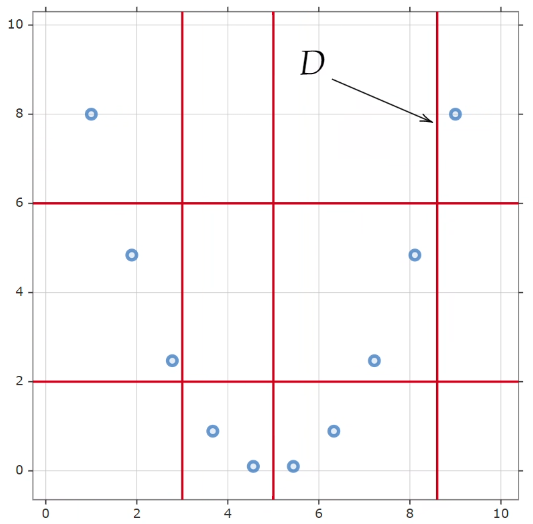
\includegraphics[scale = 0.4]{mallaG4x3.png}
            \caption{Malla G de 4x3 sobre el conjunto de pares ordenados D}
            \label{mallaG}
        \end{figure}
    
        Para la Figura \ref{mallaG}, la funci\'on de densidad quedar\'ia de la forma:

        \begin{equation}
            \label{eq:funcion_densidad}
            f_{D|_G}(i,j) = \left\{\begin{array}{lr}
                \frac{1}{10} & \text{si } (i,j) \in \{ (1,3), (4,1)\} \\
                \frac{2}{10}, & \text{si }(i,j) \in \{ (1,2), (2,1), (3,1),(3,2)\}  \\
                0, & \text{Otro caso.}
                \end{array}\right.
        \end{equation}
    
    
        Notemos que para un $D$ fijo, aunque fijemos el grosor de la malla, la distribuci\'on de esta puede variar dependiendo de donde hagamos los cortes, por ejemplo:
    
        \begin{figure}[H] 
            \centering
            \includegraphics*[scale = 0.4]{mallaG4x3_2.png}
            \caption{Otra malla G de 4x3 sobre el conjunto de pares ordenados D.}
            \label{malla_G_2}
        \end{figure}
    
        Aqu\'i podemos ver que la funci\'on de densidad que nos entrega est\'a malla es distinta a la definida para la Figura \ref{malla_G_2} . Este es un hecho que explotamos en la siguiente definici\'on: 
    
        \begin{defn}
            Para un conjunto finito $D\in\R^2$ y enteros positivos $i,j$, definimos:
            $$
            I^*(D,i,j)=\max I(D|_G),
            $$
            donde el m\'aximo es sobre todas las mallas $G$ con $i$ columnas y $j$ filas, con $I(D|_G)$ denota la informaci\'on mutua de $D|_G$.
        \end{defn}
    
        \begin{rem}
            Aunque la cantidad de mallas en la pr\'actica es infinita, tenemos una cantidad finita de pares de datos, por lo que la cantidad de distribuciones como se muestra en la ecuaci\'on \ref{eq:funcion_densidad} deben ser finitas, por lo que el m\'aximo est\'a bien definido, puesto que dos mallas que generan la misma distribuci\'on de probabilidad se consideran la misma.
        \end{rem}

        Ya teniendo este valor procedemos a definir la matriz caracteristica del conjunto $D$.
    
        \begin{defn}
            La matriz caracteristica $M(D)$ de un conjunto de pared ordenados $D$ es una matriz infinita con entradas:
            $$
            M(D)_{x, y}=\frac{I^{*}(D, x, y)}{\log \min \{x, y\}}.
            $$
        \end{defn}

        Y con esto, ya estamos listos para definir el coeficiente de informaci\'on m\'axima.

        \begin{defn}
            El coeficiente de informaci\'on m\'axima o \textit{MIC} de un conjunto bivariado $D$ de tama\~no $n$ y una malla de tama\~no menor a $B(n)$ esta dado por:
    
            $$
            \operatorname{MIC}(D)=\max _{x y<B(n)}\left\{M(D)_{x, y}\right\},
            $$
    
            donde $\omega(1)<B(n) \leq O\left(n^{1-\varepsilon}\right)$ para alg\'un $0<\varepsilon<1$.
        \end{defn}
        \begin{rem}
            A menos que se especifique de otra forma, al momento de trabajar con esta medida usaremos $B(n)=n^{0.6}$, funci\'on de la cu\'al se encontr\'o que funcon\'a en pr\'actica en el art\'iculo complementario de Reshef et al. (2011) \cite[]{Reshef2011}, discuteremos la selecci\'on de este par\'ametro m\'as adelante en \ref{eligiendo_Bn}
        \end{rem}
    
    
        \subsection[Formas practicas de calcular el MIC.]{Formas pr\'acticas de calcular el $MIC$.}

        A pesar que el $MIC$ tiene una definici\'on relativamete simple, resulta que su c\'alculo es tremeandamente complejo, dado que se debe buscar un m\'aximo en el espacio de busqueda de las mallas $G$. En el paper de Reshef et al. (2011) \cite{Reshef2011} se propone un algoritmo heur\'istico para calcular el $MIC$, llamado \textit{Approx-MIC}, que consiste en un algoritmo de b\'usqueda local que busca el m\'aximo de la matriz caracter\'istica. Este algoritmo es r\'apido y eficiente, pero no garantiza encontrar el m\'aximo global, por lo que no es un estimador consistente del $MIC$.
    
        En el art\'iculo "Measuring Dependence Powerfully and Equitably" de Reshef et al. \cite{Reshef2016}, los autores presentan y caracterizan te\'oricamente dos nuevas medidas de dependencia: $MIC_*$ y $MIC_e$. $MIC_*$ es una medida de dependencia poblacional, y el art\' iculo presenta tres formas de ver esta cantidad. Los autores demuestran que $MIC_*$ es el valor poblacional del coeficiente de informaci\'on m\'axima (MIC), una suavizaci\'on m\'inima de la informaci\'on mutua y el supremo de una secuencia infinita. Estas caracterizaciones simplifican el c\'alculo y fortalecen los resultados te\'oricos.
    
        Adem\'as, los autores desarrollan algoritmos eficientes para aproximar $MIC_*$ en la pr\'actica y estimarlo de manera consistente a partir de una muestra finita. Introducen $MIC_e$, un estimador consistente de $MIC_*$, que es computable de manera eficiente y m\'as r\'apido en la pr\'actica que el algoritmo heur\'istico para calcular MIC. A trav\'es de simulaciones, demuestran que $MIC_e$ tiene mejores propiedades de sesgo/varianza y supera a los m\'etodos existentes en t\'erminos de equitabilidad con respecto a R2 en un amplio conjunto de relaciones funcionales ruidosas.

        El resto de la secci\'on est\'a dedicado a presentar las definiciones y propiedades de $MIC_*$ y $MIC_e$, la relaci\'on entre ellos y el con el $MIC$, y c\'omo se pueden calcular en la pr\'actica.
    
        \subsubsection{Definiciones y propiedades de $MIC_*$}
    
        El coeficiente m\'aximo de informaci\'on poblacional o $MIC_*$ puede expresarse de diversas maneras equivalentes, como veremos m\'as adelante. Sin embargo, comenzaremos con la definici\'on m\'as sencilla.
    
        \begin{defn}[$MIC_*$]
            Sea $(X,Y)$ un vector aleatorio bivariado. El coeficiente de informaci\'on m\'axima poblacional ($MIC_*$) de $(X,Y)$ se define como:
            $$
            M I C_*(X, Y)=\sup _G \frac{I\left(\left.(X, Y)\right|_G\right)}{\log \|G\|},
            $$
            
            donde $||G||$ denota el m\'inimo entre el n\'umero de filas y el n\'umero de columnas de la malla $G$.
        \end{defn}
        
        Ya que $I(X,Y) = sup_G I((X,Y)|G)$ (Cover y Thomas, 2006 \cite[Cap. 8]{CoverThomas2006}), esto puede interpretarse como una versi\'on regularizada de la informaci\'on mutua que sanciona las rejillas complejas y garantiza que el resultado est\'e dentro del rango entre cero y uno.
        
        Previo a continuar, introducimos una definici\'on equivalente y sencilla de $MIC_*$ que resulta \'util para los resultados en esta secci\'on. Esta definici\'on considera a $MIC_*$ como el supremo de una matriz denominada matriz caracter\'istica poblacional, que se define a continuaci\'on.
        
        \begin{defn}[Matriz caracter\'istica poblacional]
            Sea $(X,Y)$ vector aleatorio bivariado. Sea
            $$
            I^*((X, Y), k, \ell)=\max _{G \in G(k, \ell)} I\left(\left.(X, Y)\right|_G\right),
            $$
            la matriz caracter\'istica poblacional de (X,Y), denotada por M(X,Y), se define como
            $$
            M(X, Y)_{k, \ell}=\frac{I^*((X, Y), k, \ell)}{\log \min \{k, \ell\}}.
            $$
        \end{defn}
        
        para $k$, $l > 1$.
        
        Es f\'acil ver lo siguiente:
    
        \begin{prop}
            Sea $(X,Y)$ vector aleatorio bivariado. Tenemos
        
        $$MIC_*(X,Y) = \sup M(X,Y),$$
        
        donde $M(X,Y)$ es la matriz caracter\'istica poblacional de $(X,Y)$.
        \end{prop}	
    
        
        La matriz caracter\'istica poblacional recibe este nombre porque, al igual que el $MIC_*$, el supremo de esta matriz, captura una noci\'on de la intensidad de la relaci\'on, y otras propiedades de esta matriz se relacionan con diferentes caracter\'isticas de las relaciones. Por ejemplo, m\'as adelante en este documento presentamos una propiedad adicional de la matriz caracter\'istica, el coeficiente de informaci\'on total, que es \'util para comprobar la presencia o ausencia de una relaci\'on en lugar de cuantificar la intensidad de la relaci\'on.
    
        \subsubsection[]{El $MIC_*$ es el valor poblacional del $MIC$}
    
        Con el $MIC_*$ definido, presentamos nuestra primera caracterizaci\'on alternativa de este, como el l\'imite de muestra grande del estad\'istico MIC introducido en Reshef et al. \cite{Reshef2011}. Notemos que para evistar confuci\'on denotaremos como $MIC$ al estad\'istico MIC y como $MIC_*$ al coeficiente de informaci\'on m\'axima poblacional.
    
        El siguiente resultado, demostrado en el paper de Reshef (2'16)\cite{Reshef2016}, sobre la convergencia de funciones de la matriz caracter\'istica de muestra a sus contrapartes poblacionales, una consecuencia de lo cual es la convergencia de MIC a $MIC_*$. (En la declaraci\'on del teorema a continuaci\'on, recordemos que $m_\infty$ es el espacio de matrices infinitas equipadas con la norma supremo, y dada una matriz A, la proyecci\'on ri anula todas las entradas $A_{k, \ell}$ para las cuales $k\ell > i.$)
    
        \begin{thm}
            Sea $f: m^{\infty} \rightarrow \mathbb{R}$ uniformemente continua, y suponga que $f \circ r_i \rightarrow f$ puntualmente. Entonces, para cada variable aleatoria $(X, Y)$, tenemos
            $$
            \left(f \circ r_{B(n)}\right)\left(\widehat{M}\left(D_n\right)\right) \rightarrow f(M(X, Y)),
            $$
            en probabilidad donde $D_n$ es una muestra de tama\~no $n$ de la distribuci\'on de $(X, Y)$, siempre que $\omega(1)<B(n) \leq O\left(n^{1-\varepsilon}\right)$ para alg\'un $\varepsilon>0$.
        \end{thm}
    
        Dado que el supremo de una matriz es una funci\'on uniformemente continua en $m_\infty$ y se puede realizar como el l\'imite de m\'aximos de segmentos cada vez m\'as grandes de la matriz, este teorema genera nuestra afirmaci\'on sobre $MIC_*$ como corolario.
    
        \begin{cor}
            $MIC$ es un estimador consistente de $MIC_*$ siempre que $\omega(1) < B(n) \leq O(n^{1-\epsilon})$ para alg\'un $\epsilon > 0$
        \end{cor}
    
        Con esto podemos trabajar, bajo ciertas condiciones, con el $MIC_*$ como reemplazo del $MIC$. Pero, ¿Cu\'al es la ventaja de trabajar con este nuevo estimador? En pocas palabras, es m\'as f\'acil de estimar, y esto lo veremos en la en una secci\'on m\'as adelante. Antes de esto debemos revisar una caracterizaci\'on del $MIC_*$ que nos permitir\'a contruir un estimador de este.
    
        \subsubsection[El MIC star es el supremo de la matriz caracteristica de muestra]{El $MIC_*$ es el supremo de la matriz caracter\'istica de muestra}
    
        Ahora mostramos la una vista alternativa de $MIC_*$: que puede definirse de manera equivalente como el supremo sobre la frontera de la matriz caracter\'istica en lugar de como un supremo sobre todas las entradas de la matriz. Esta caracterizaci\'on de $MIC_*$ servir\'a como base tanto para la aproximaci\'on de $MIC_*(X, Y)$ como para el nuevo estimador de $MIC_*$ ser\'a presentado m\'as adelante.
    
        Comenzamos definiendo lo que entendemos por frontera de la matriz caracter\'istica. Nuestra definici\'on se basa en la siguiente observaci\'on.
        \begin{prop}
            Sea $M$ una matriz caracter\'istica poblacional. Entonces, para $\ell \geq k, M_{k, \ell} \leq M_{k, \ell+1}$.
        \end{prop}
        \begin{proof}
            Sea $(X, Y)$ la variable aleatoria en cuesti\'on. Siempre podemos dejar una fila/columna vac\'ia, sabemos que $I^*((X, Y), k, \ell) \leq I^*((X, Y), k, \ell+1)$. Y dado que $\ell, \ell+1 \geq k$, sabemos que $M_{k, \ell}=I^*((X, Y), k, \ell) / \log k \leq I^*((X, Y), k, \ell+1) / \log k=M_{k, \ell+1}$.
        \end{proof}
    
        Dado que las entradas de la matriz caracter\'istica est\'an acotadas, el teorema de convergencia mon\'otona nos da el siguiente corolario. En el corolario y en adelante, dejamos $M_{k, \uparrow}=\lim _{\ell \rightarrow \infty} M_{k, \ell}$ y definimos $M_{\uparrow, \ell}$ de manera similar.

        \begin{cor}
            Sea $M$ una matriz caracter\'istica poblacional. Entonces, $M_{k, \uparrow}$ existe, es finito e igual a $\sup _{\ell \geq k} M_{k, \ell}$. Lo mismo es v\'alido para $M_{\uparrow, \ell}$. \label{cor:frontera}
        \end{cor}
    
        El corolario anterior nos permite definir la frontera de la matriz caracter\'istica.
    
        \begin{defn}
            Sea $M$ una matriz caracter\'istica poblacional. La frontera de $M$ es el conjunto
            $$
            \partial M=\left\{M_{k, \uparrow}: 1<k<\infty\right\} \bigcup\left\{M_{\uparrow, \ell}: 1<\ell<\infty\right\}.
            $$
        \end{defn}
        
        El teorema siguiente da una relaci\'on entre la frontera de la matriz caracter\'istica y $\mathrm{MIC}_*$.
        
        
        \begin{thm}
            Sea $(X, Y)$ un vector aleatorio bivariado. Tenemos
            $$
            M I C_*(X, Y)=\sup \partial M(X, Y),
            $$
            donde $M(X, Y)$ es la matriz caracter\'istica poblacional de $(X, Y)$.
        \end{thm}
    
    
        \begin{proof}
            El siguiente argumento muestra que cada entrada de $M$ es, como m\'aximo, $\sup \partial M$: fije un par $(k, \ell)$ y observe que, o bien $k \leq \ell$, en cuyo caso $M_{k, \ell} \leq M_{k, \uparrow}$, o bien $\ell \leq k$, en cuyo caso $M_{k, \ell} \leq M_{\uparrow, \ell}$. 
            
            Por lo tanto, $\mathrm{MIC}_* \leq \sup \left\{M_{\uparrow, \ell}\right\} \cup\left\{M_{k, \uparrow}\right\}=\sup \partial M$.
        \end{proof}
        
        Por otro lado, el Corolario \ref{cor:frontera} muestra que cada elemento de $\partial M$ es un supremo sobre algunos elementos de $M$. Por lo tanto, sup $\partial M$, al ser un supremo sobre supremos de elementos de $M$, no puede exceder $\sup M=\mathrm{MIC}_*$.
    
    
        \subsubsection[Estimando el MIC* con MICe]{Estimando $MIC_*$ con $MIC_e$}
    
    
        El estimador $MIC_e$ se basa en la caracterizaci\'on alternativa de $MIC_*$ probada en la secci\'on anterior, si $MIC_*$ puede considerarse como el supremo del l\'imite de la matriz caracter\'istica en lugar de la matriz completa, entonces solo el l\'imite de la matriz debe estimarse con precisi\'on para estimar $MIC_*$. Esto tiene la ventaja de que, mientras que calcular entradas individuales de la matriz caracter\'istica de muestra implica encontrar mallas \'optimas (bidimensionales), estimar las entradas del l\'imite nos requiere solo encontrar particiones \'optimas (unidimensionales). Si bien el primer problema es computacionalmente dif\'icil, el segundo puede resolverse utilizando el algoritmo de programaci\'on din\'amica de Reshef et al.(2011)\cite{Reshef2011}.
    
        En Reshef (2016) \cite{Reshef2016}, esta idea es formalizada a travez de un objeto llamado la matriz equicaracter\'istica, la cual es denominadad $[M]$. La diferencia entre $[M]$ y la matriz caracter\'istica $M$ es la siguiente: mientras que la entrada $k, \ell$-\'esima de $M$ se calcula a partir de la informaci\'on mutua m\'axima alcanzable utilizando cualquier cuadr\'icula de $k\times\ell$, la entrada $k, \ell$-\'esima de $[M]$ se calcula a partir de l\ informaci\'on mutua m\'axima alcanzable utilizando cualquier cuadr\'icula de $k\times\ell$ que equiparticiona la dimensi\'on con m\'as filas/columnas (Ver Figura \ref{fig:matriz_equicaracteristica}.) A pesar de esta diferencia, a medida que la equipartici\'on en cuesti\'on se vuelve m\'as y m\'as fina, se vuelve indistinguible de una partici\'on \'optima del mismo tama\~no Esta intuici\'on se puede formalizar para mostrar que el l\'imite de $[M]$ es igual al l\'imite de $M$, y por lo tanto que $\sup [M]=\sup M=\mathrm{MIC}*$. Entonces, se deducir\'a que estimar $[M]$ y tomar el supremo, como lo hicimos con $M$ en el caso de MIC, proporciona una estimaci\'on consistente de $\mathrm{MIC}*$.
    
        \subsection{La matriz equicaracter\'istica} 
    
        Ahora definimos la matriz equicaracter\'istica y mostramos que su supremo es efectivamente $MIC^*$. Para hacerlo, primero definimos una versi\'on de $I^*$ que equiparticiona la dimensi\'on con m\'as filas/columnas. Observe que en la definici\'on, los corchetes se utilizan para indicar la presencia de una equipartici\'on.
    
        \begin{figure} 
            \centering
            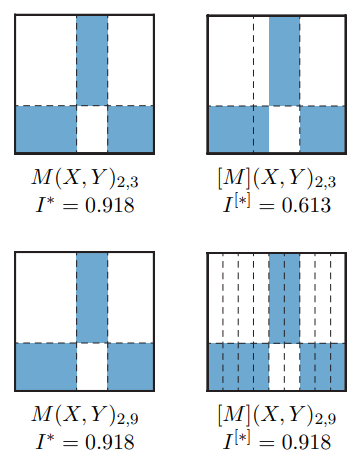
\includegraphics[scale=0.8]{figuras/figure_1_reshef_2016.png}
            \caption{Un esquema que ilustra la diferencia entre la matriz caracter\'istica $M$ y la matriz equicaracter\'istica $[M]$. (Arriba) Cuando se restringe a 2 filas y 3 columnas, la matriz caracter\'istica $M$ se calcula a partir de la rejilla \'optima de 2 por 3. En contraste, la matriz equicaracter\'istica $[M]$ a\'un optimiza la partici\'on m\'as peque\~na de tama\~no 2 pero est\'a restringida a tener la partici\'on m\'as grande como una equipartici\'on de tama\~no 3. Esto resulta en una informaci\'on mutua m\'as baja de 0.613. (Abajo) Cuando se permiten 9 columnas en lugar de 3, la rejilla encontrada por la matriz caracter\'istica no cambia, ya que la rejilla con 3 columnas ya era \'optima. Sin embargo, ahora la matriz equicaracter\'istica utiliza una equipartici\'on en columnas de tama\~no 9, cuya resoluci\'on es capaz de capturar completamente la dependencia entre $X$ e $Y$.}
            \label{fig:matriz_equicaracteristica}
        \end{figure}
        
    
        \begin{defn}
            Sea $(X, Y)$ variables aleatorias conjuntamente distribuidas. Definir
            $$
            I^*((X, Y), k,[\ell])=\max _{G \in G(k,[\ell])} I\left(\left.(X, Y)\right|_G\right),
            $$
            donde $G(k,[\ell])$ es el conjunto de mallas de $k$ por $[\ell]$ cuya partici\'on del eje $y$ es una equipartici\'on de tama\~no $\ell$. Definir $I^*((X, Y),[k], \ell)$ an\'alogamente.
    
            Definir $I^{[*]}((X, Y), k, \ell)$ igual a $I^((X, Y), k,[\ell])$ si $k<\ell$ y $I^*((X, Y),[k], \ell)$ en otro caso.
        \end{defn}
    
        Ahora definimos la matriz equicaracter\'istica en t\'erminos de $I^{[*]}$. En la definici\'on a continuaci\'on, continuamos nuestra convenci\'on de usar corchetes para denotar la presencia de equiparticiones.
    
        \begin{defn}
            Sea $(X, Y)$ variables aleatorias conjuntamente distribuidas. La matriz equicaracter\'istica de poblaci\'on de $(X, Y)$, denotada por $[M](X, Y)$, se define por
            $$
            [M](X, Y)_{k, \ell}=\frac{I^{[*]}((X, Y), k, \ell)}{\log \min \{k, \ell\}},
            $$
            para $k, \ell>1$.
        \end{defn}
    
        La frontera de la matriz equicaracter\'istica se puede definir mediante un l\'imite de la misma manera que la matriz caracter\'istica. Luego tenemos el siguiente teorema.
    
        \begin{thm}
            Sea $(X, Y)$ variables aleatorias conjuntamente distribuidas. Entonces $\partial[M]=\partial M$.
        \end{thm}
        \begin{proof}
            Ap\'endice F de Reshef 2016
        \end{proof}
    
        Dado que cada entrada de la matriz equicaracter\'istica est\'a dominada por alguna entrada en su frontera, la equivalencia de $\partial[M]$ y $\partial M$ produce el siguiente corolario como una simple consecuencia.
    
        \begin{cor}
            Sea $(X, Y)$ variables aleatorias conjuntamente distribuidas. Entonces $\sup [M](X, Y)=$ $M I C_*(X, Y)$.
        \end{cor}
    
        \subsection[short]{El estimador $MIC_e$}
    
        Con la matriz equicaracter\'istica definida, podemos ahora definir nuestro nuevo estimador $\mathrm{MIC}_e$ en t\'erminos de la matriz equicaracter\'istica de muestra, de manera an\'aloga a c\'omo definimos MIC con la matriz caracter\'istica de muestra.
    
        \begin{defn}
            Sea $D \subset \mathbb{R}^2$ un conjunto de pares ordenados. La matriz equicaracter\'istica de muestra $\widehat{[{M}]}(D)$ de $D$ se define como
            $$
            \widehat{[{M}]}(D)_{k, \ell}=\frac{I^{[*]}(D, k, \ell)}{\log \min \{k, \ell\}} .
            $$
        \end{defn}
        \begin{defn}
            Sea $D \subset \mathbb{R}^2$ un conjunto de $n$ pares ordenados, y sea $B: \mathbb{Z}^{+} \rightarrow \mathbb{Z}^{+}$. Definimos
            $$
            M I C_{e, B}(D)=\max _{k \ell \leq B(n)} \widehat{[M]}(D)_{k, \ell}.
            $$
        \end{defn}
    
    
        Con la equivalencia establecida entre la frontera de la matriz caracter\'istica y el de la matriz equicaracter\'istica, es f\'acil demostrar que $\mathrm{MIC}e$ es un estimador consistente de $\mathrm{MIC}*$ mediante argumentos similares a los que aplicamos en el caso de MIC. (Ver Ap\'endice G. Reshef (2016)\cite{Reshef2016}) Espec\'ificamente, mostramos el siguiente teorema, un an\'alogo del Teorema 6.
        
        \begin{thm}
            Sea $f: m^{\infty} \rightarrow \mathbb{R}$ uniformemente continua, y suponga que $f \circ r_i \rightarrow f$ puntualmente. Entonces para cada variable aleatoria $(X, Y)$, tenemos:
    
            $$
            \left.\left(f \circ r_{B(n)}\right)(\widehat{M}]\left(D_n\right)\right) \rightarrow f([M](X, Y)),
            $$
    
            en probabilidad donde $D_n$ es una muestra de tama\~no $n$ de la distribuci\'on de $(X, Y)$, siempre que $\omega(1)<B(n) \leq O\left(n^{1-\varepsilon}\right)$ para alg\'un $\varepsilon>0$.
        \end{thm}
        \begin{proof}
            Ap\'endice A. Reshef (2016) \cite{Reshef2016}
        \end{proof}
    
        Al establecer $f([M])=\sup [M]$, obtenemos como corolario la consistencia de $\mathrm{MIC}_e$.
        
        \begin{cor}
            $M I C_{B}$ es un estimador consistente de $M I C_*$ siempre que $\omega(1)<B(n) \leq O\left(n^{1-\varepsilon}\right)$ para alg\'un $\varepsilon>0$.
        \end{cor}
    
        \subsubsection[computando mic e ]{Computando $MIC_e$}
    
        Tanto el $MIC$ como el $MIC_e$ son estimadores consistentes de $MIC_*$. La diferencia entre ellos radica en que, mientras que el $MIC$ actualmente solo se puede calcular de manera eficiente a trav\'es de una aproximaci\'on heur\'istica, el $MIC_e$ se puede calcular de manera exacta y muy eficiente mediante un enfoque similar al utilizado para aproximar $MIC_*$ que involucra la subrutina \textit{OptimizeXAxis}. Ahora repasaremos los detalles de este enfoque.
    
        Recordemos que, dada una partici\'on fija del eje $x$ $Q$ en $\ell$ columnas, un conjunto de $n$ puntos de datos, una partici\'on ''maestra'' del eje $y$ $\Pi$, y un n\'umero $k$, la subrutina \textit{OptimizeXAxis} encuentra, para cada $2 \leq i \leq k$, una partici\'on del eje $y$ $P_i \subset \Pi $ de tama\~no como m\'aximo $i$ que maximiza la informaci\'on mutua inducida por la cuadr\'icula $(P_i, Q)$. El algoritmo realiza esto en un tiempo de $O(|\Pi|^2k\ell)$. Para obtener m\'as detalles sobre \textit{OptimizeXAxis}, consulte la Secci\'on 3.5 de Reshef el al. (2016) \cite{Reshef2016} 
    
        En el par de teoremas a continuaci\'on, se muestran dos formas en que \textit{OptimizeXAxis} se puede utilizar para calcular eficientemente el $MIC_e$. 
    
        \begin{thm}
    
            Existe un algoritmo  \textit{EQUICHAR} que, dada una muestra $D$ de tama\~no $n$ y alg\'un $B \in \mathbb{Z}^{+}$, computa la porci\'on $r_{B(n)}(\widehat{[M]}(D))$ de la matriz equicaracteristica poblacional en tiempo $O\left(n^2 B^2\right)$, que es equivalente a $O\left(n^{4-2 \varepsilon}\right)$ para $B(n)=O\left(n^{1-\varepsilon}\right)$ con $\varepsilon>0$.
        \end{thm}
    
        \begin{proof}
            Describimos el algoritmo y simult\'aneamente acotamos su tiempo de ejecuci\'on. Lo hacemos \'unicamente para las entradas $k, \ell$-\'esimas de $\widehat{[M]}(D)$ que satisfacen $k \leq \ell, k \ell \leq B$. Esto es suficiente, ya que por simetr\'ia, calcular el resto de las entradas requeridas como m\'aximo duplica el tiempo de ejecuci\'on.
    
            Para calcular $\widehat{[M]}(D)_{k, \ell}$ con $k \leq \ell$, debemos fijar una partici\'on equitativa en $\ell$ columnas en el eje $\mathrm{x}$ y luego encontrar la partici\'on \'optima del eje $\mathrm{y}$ de tama\~no como m\'aximo $k$. Si configuramos la partici\'on maestra $\Pi$ del algoritmo \textit{OptimizeXAxis} como una partici\'on equitativa en filas de tama\~no $n$, entonces realiza precisamente la optimizaci\'on requerida. Adem\'as, para un $\ell$ fijo, puede llevar a cabo la optimizaci\'on simult\'aneamente para todos los pares ${(2, \ell), \ldots,(B / \ell, \ell)}$ en tiempo $O\left(|\Pi|^2(B / \ell) \ell\right)=O\left(n^2 B\right)$. Para un $\ell$ fijo, este conjunto contiene todos los pares $(k, \ell)$ que satisfacen $k \leq \ell, k \ell \leq B$. Por lo tanto, para calcular todas las entradas requeridas de $\widehat{[M]}(D)$, solo necesitamos aplicar este algoritmo para cada $\ell=2, \ldots, B / 2$. Hacerlo resulta en un tiempo de ejecuci\'on de $O\left(n^2 B^2\right)$.
        \end{proof}
    
        El algoritmo mencionado anteriormente, aunque es de tiempo polin\'omico, no es lo suficientemente eficiente para su uso en la pr\'actica. Sin embargo, una modificaci\'on simple resuelve este problema sin afectar la consistencia de las estimaciones resultantes. La modificaci\'on se basa en el hecho de que OptimizeXAxis puede usar particiones maestras $\Pi$ adem\'as de la partici\'on equitativa de tama\~no $n$ que utilizamos anteriormente. Espec\'ificamente, configurar $\Pi$ en el algoritmo anterior como una partici\'on equitativa en $c k$ "grupos", donde $k$ es el tama\~no de la partici\'on \'optima m\'as grande que se est\'a buscando, acelera significativamente el c\'alculo. Esta modificaci\'on proporciona una estad\'istica ligeramente diferente, pero que tiene todas las propiedades te\'oricas de $\mathrm{MIC}e$, es decir, una estimaci\'on consistente de $\mathrm{MIC}*$ y un c\'alculo exacto eficiente. Estas propiedades se formalizan en el siguiente teorema
    
        \begin{thm}
            Sea $(X, Y)$  un vertor aleatorio bivariado, y sea $D_n$ y sea una muestra de tama\~no $n$ de la distribuci\'on $(X, Y)$. Para cada $c \geq 1$, existe una matriz $\{\widehat{M}\}^c\left(D_n\right)$ tal que:
            \begin{enumerate}
                \item La funci\'on
                $$
                \widetilde{M I C_{e, B}}(\cdot)=\max {k \ell \leq B(n)}\{\widehat{M}\}^c(\cdot){k, \ell},
                $$
                es un estimador concistente de $M I C_*$ dado $\omega(1)<B(n) \leq O\left(n^{1-\varepsilon}\right)$ para alg\'un $\varepsilon>0$.
                2. Existe un algoritmo \textit{EQUICHARCLUMP} para comparar $r_B\left(\{\widehat{M}\}^c\left(D_n\right)\right)$ en tiempo $O\left(n+B^{5 / 2}\right)$, que equivale a $O\left(n+n^{5(1-\varepsilon) / 2}\right)$ cuando $B(n)=O\left(n^{1-\varepsilon}\right)$.
            \end{enumerate}
        \end{thm}
        \begin{proof}
            Ap\'endice H. Reshef (2016) \cite{Reshef2016}
        \end{proof}

        Para un an\'alisis del efecto del par\'ametro $c$ en el teorema anterior en los resultados del algoritmo \textit{EQUICHARCLUMP}, consulte el Ap\'endice H.3 de Reshef el al. (2016) \cite{Reshef2016}. Estableciendo $\varepsilon=0.6$ en el teorema anterior, obtenemos el siguiente corolario.

        \begin{cor}
            $ M I C_*$ puede estimarse de manera consistente en tiempo lineal. 
        \end{cor}

        Por supuesto, en tama\~nos de muestra peque\~nos, establecer $\varepsilon=0.6$ ser\'ia indeseable. Sin embargo, en el art\'iculo complementario (Reshef et al.,(2015a) \cite{Reshef2015a}) demuestra emp\'iricamente que en tama\~nos de muestra grandes, esta estrategia funciona muy bien en relaciones t\'ipicas.

        Cabe destacar que el algoritmo \textit{EQUICHARCLUMP} dado anteriormente es asint\'oticamente m\'as r\'apido incluso que el algoritmo heur\'istico \textit{APPROX-MIC} utilizado para calcular MIC en la pr\'actica, que se ejecuta en tiempo $O\left(B(n)^4\right)$. Como se demostr\'o en el art\'iculo complementario (Reshef et al., 2015a \cite{Reshef2016}), esta diferencia se traduce en una diferencia sustancial en los tiempos de ejecuci\'on para un rendimiento similar en una gama de tama\~nos de muestra realistas, que va desde una aceleraci\'on de 30 veces en $n=500$ hasta m\'as de 350 veces en $n=10,000$.
    
    
        \subsubsection[eligiendoBn]{Eligiendo $B(n)$}\label{eligiendo_Bn}
            
        Recordemos que, como fue propuesto en Reshef el al. (2011) \cite{Reshef2011}, utilizamos funciones de la forma $B(n)=n^\alpha$. Valores grandes de $\alpha$ conducen a un aumento en el error esperado en reg\'imenes de baja se\~nal ($R^2$ bajos) debido tanto a un sesgo positivo en esos reg\'imenes como a un aumento general en la varianza que afecta predominantemente a esos reg\'imenes. Por otro lado, valores peque\~nos de $\alpha$ llevan a un aumento en el error esperado en reg\'imenes de alta se\~nal (R2 altos) al generar un sesgo negativo en esos reg\'imenes y desplazar la varianza del estimador hacia esos reg\'imenes. En otras palabras, valores m\'as bajos de $\alpha$ son m\'as adecuados para detectar se\~nales m\'as d\'ebiles, mientras que valores m\'as altos de $\alpha$ son m\'as adecuados para distinguir entre se\~nales m\'as fuertes. Esto concuerda con los resultados observados en el trabajo complementario (Reshef et al., (2015a) \cite{Reshef2015a} ), que muestran que valores bajos de $\alpha$ hacen que MICe proporcione pruebas de independencia con mejor potencia, mientras que valores altos de $\alpha$ hacen que MICe tenga una mejor equidad.
    
    
        \subsection[TIC]{\textit{Total Information coefficient ($TIC$)}}
    
        Hasta ahora hemos presentado resultados sobre estimadores del coeficiente de informaci\'on maximal de la poblaci\'on, una cantidad para la cual la equitabilidad es la principal motivaci\'on. Ahora introducimos y analizamos una nueva medida de dependencia, el coeficiente de informaci\'on total ($TIC$). A diferencia del coeficiente de informaci\'on maxima ($MIC$), el coeficiente de informaci\'on total no est\'a dise\~nado para la equitabilidad, sino m\'as bien como una estad\'istica de prueba para probar una hip\'otesis nula de independencia.
    
        Comenzamos dando alguna intuici\'on. Recordemos que el coeficiente de informaci\'on maximal es el supremo de la matriz caracter\'istica. Si bien estimar el supremo de esta matriz tiene muchas ventajas, esta estimaci\'on implica tomar un m\'aximo sobre muchas estimaciones de las entradas individuales de la matriz caracter\'istica. Dado que los m\'aximos de conjuntos de variables aleatorias tienden a aumentar a medida que crece el n\'umero de variables, se puede imaginar que este procedimiento puede llevar a un sesgo positivo indeseable en el caso de la independencia estad\'istica, cuando la matriz caracter\'istica de la poblaci\'on es igual a 0. Esto podr\'ia ser perjudicial para las pruebas de independencia, donde la distribuci\'on muestral de una estad\'istica bajo una hip\'otesis nula de independencia es crucial.
        
        La intuici\'on detr\'as del coeficiente de informaci\'on total es que si en cambio consideramos una propiedad m\'as estable, como la suma de las entradas en la matriz caracter\'istica, podr\'iamos esperar obtener una estad\'istica con un sesgo m\'as peque\~no en el caso de independencia y, por lo tanto, una mejor potencia. En resumen, si nuestro \'unico objetivo es distinguir cualquier dependencia de ruido completo, entonces ignorar toda la matriz caracter\'istica de la muestra, excepto su valor m\'aximo, puede descartar una se\~nal \'util, y el coeficiente de informaci\'on total evita esto al sumar todas las entradas.
        
        Cabe destacar que en Reshef et al. (2011)\cite{Reshef2011} se sugiere que otras propiedades de la matriz caracter\'istica pueden permitirnos medir otros aspectos de una relaci\'on dada adem\'as de su fuerza, y se definieron varias de estas propiedades. El coeficiente de informaci\'on total encaja dentro de este marco conceptual. En la siguiente secci\'on definimos el coeficiente de informaci\'on total en el caso de la matriz caracter\'istica ($TIC$) y la matriz equicaracter\'istica ($TIC_e$). Luego demostramos que tanto TIC como TICe producen pruebas de independencia que son consistentes frente a todas las alternativas dependientes. (Al igual que en el caso de $MIC$ y $MIC_e$, $TIC_e$ es m\'as f\'acil de calcular que $TIC$). Finalmente, revisaremos un estudio de simulaci\'on sobre la potencia de las pruebas de independencia basadas en TICe realizado en el paper de Reshef (2016)\cite{Reshef2016} en un conjunto de relaciones elegidas en Simon y Tibshirani (2012)\cite[]{SimonTibshirani}, mostrando que $TIC_e$ supera a otras medidas comunes de dependencia en muchas de las relaciones y se ajusta estrechamente a su rendimiento en el resto.
    
    
        \subsection[definicionyconcitenciatic]{Definici\'on y Consistenc\'ia de TIC}
    
        Comenzamos definiendo dos versiones del coeficiente. En la siguiente definici\'on notemos qu\'e $\widehat{M}$ denota la matriz caracteristica poblacional y $\widehat{[M]}$ denota la matriz equicaracteristica de poblacional.
    
        \begin{defn}
            Sea $D \subset \mathbb{R}^2$ un conjunto de $n$ pares ordenados, y sea $B: \mathbb{Z}^{+} \rightarrow \mathbb{Z}^{+}$. Definimos:
            $$
            T I C_B(D)=\sum_{k \ell \leq B(n)} \widehat{M}(D)_{k, \ell},
            $$
            y
            $$
            T I C_{e, B}(D)=\sum_{k \ell \leq B(n)} \widehat{[M]}(D)_{k, \ell}.
            $$
        \end{defn}
    
        Ahora nos interesa mostrar que estos estad\'isticos nos entregan test de independencia concistente, para esto debemos detenernos y analizar el comportamiento de las cantidades poblacionales an\'alogas. 
    
        \begin{defn}
            Para una matriz $A$	y un n\'umero positivo $B$, la $B$-parcial suma de 	$A$, denotada por  $S_B(A)$, es:
            $$
            S_B(A)=\sum_{k \ell \leq B} A_{k, \ell}.
            $$
            
            Cuando $A$ es una matriz (equi)caracteristica, $S_B(A)$ es la suma sobre todas las entradas correpondientes a mallas con al menos $B$ celdas totales. Por tanto, si $\widehat{M}(D)$ es una matriz equicaracteristica poblacional de $D, S_B(\widehat{M}(D))=\mathrm{TIC}_B(D)$, y lo mismo se mantiene cierto para $S_B(\widehat{[M]}(D))$ and $\mathrm{TIC}_{e, B}(D)$.
            
            Es claro que si $X$ e $Y$ son variables aleatorias estad\'isticamente independientes, se tiene que ambas matrices caracteristicas $M(X, Y)$ y la matriz equicaracteristica $[M](X, Y)$ son identicamente 0 , tal que $S_B(M(X, Y))=S_B([M](X, Y))=0$ para todo $B$. Sin embargo, tambi\'en nos interesa como estas cantidades se comportan cuando las variables $X$ e $Y$ son dependietes. Las siguientes proposiciones nos ayudan a entender esto. La primera nos muestra una cota inferior para los valores de las entradas de ambas $M(X, Y)$ y $[M](X, Y)$. La segunda nos muestra una caracterizaci\'on asint\'otica de como crecen $S_B(M)$ y $S_B([M])$ como funciones de $B$. Estas dos proposiciones son el coraz\'on t\'ecnico de por qu\'e el coeficiente de informaci\'on total produce un test de independencia consistente.
            
            \begin{prop}
                Sea $(X, Y)$ un vector aleatorio bivariado. Si $X$ e $Y$ son estad\'isticamente independientes, entonces $M(X, Y) \equiv[M](X, Y) \equiv 0$. Si no, existe alg\'un $a>0$ y alg\'un entero $\ell_0 \geq 2$ tal que:
                
                $$
                M(X, Y)_{k, \ell,}[M](X, Y)_{k, \ell} \geq \frac{a}{\log \min \{k, \ell\}},
                $$
                ya sea para todo $k \geq \ell \geq \ell_0$, o para todo $\ell \geq k \geq \ell_0$.
            \end{prop}
            \begin{proof}
                Ap\'endice K.1. Reshef (2016) \cite{Reshef2016}
            \end{proof}
            \begin{prop}
                Sean $(X, Y)$ un vector aleatorio bivariado. Si $X$ e $Y$ independites, se tiene que  $S_B(M(X, Y))=S_B([M](X, Y))=0$ para todo $B>0$. Si no, tenemos que $S_B(M(X, Y))$ y $S_B([M](X, Y))$ son ambos $\Omega(B \log \log B)$.
            \end{prop}
            \begin{proof}
                Ap\'endice K.2. Reshef (2016) \cite{Reshef2016}
            \end{proof}
    
            Con las proposiciones presentadas, y siguiendo la misma l\'ogica de los argumentos de convergencia presentados anteriormente, podemos mostrar el resultado principal de esta secci\'on, que las estad\'isticas $TIC$ y $TIC_e$ producen tests de independencia consistentes.
    
            \begin{thm}
                Los estadisticos $T I C_B$ y $T I C_{e, B}$ proporcionan pruebas coherentes de cola derecha de independencia, siempre que $\omega(1)<B(n) \leq O\left(n^{1-\varepsilon}\right)$ para alg\'un $\varepsilon>0$.
            \end{thm}
            \begin{proof}
                Ap\'endice K.3. Reshef (2016) \cite{Reshef2016}
            \end{proof}
    
            En la pr\'actica, usualemente se utiliza el algoritmo  EQUICHARCLUMP \cite[Secci\'on 4.3]{Reshef2016} para computar la matriz equicaracter\'istica, de donde calculamos $\mathrm{TIC}_e$. Este algoritmo no computa la matriz equicaracteristica exactamente. Pero, como es el caso con $\mathrm{MIC}_e$, el uso del algoritmo no afecta las propiedades te\'oricas de la estad\'istica. Esta demostraci\'on se puede encontrar en Reshef el al. (2016) \cite[Ap\'endice H]{Reshef2016}
        \end{defn}
    
        \subsubsection[poder de independencia basado en TICe]{Prueba de Poder de independencia basadas en $TIC_e$}
    
        Ya sabemos que ambos, $TIC$ y $TIC_e$, son consitentes, ahora nos interesa realizar una evaluci\'on emp\'irica de la prueba de poder de independencia basado en $TIC_e$	siendo computado usando al algoritmo \textit{EQUICHARCLUMP}.
    
        En Reshef el at. (2016)\cite{Reshef2016}, para evaluar el poder que tiene esta prueba, se realiza el analisis utilizado por Simon y Tibshirani (2012) \cite{SimonTibshirani}. Este corresponde a un conjunto de relaciones definido por:
    
        $$
        \mathcal{Q}=\left\{\left(X, f(X)+\varepsilon^{\prime}\right): X \sim \text { Unif, } f \in F, \varepsilon^{\prime} \sim \mathcal{N}\left(0, \sigma^2\right), \sigma \in \mathbb{R}_{\geq 0}\right\},
        $$
        
        donde $F$ es el conjunto de relaciones definido en Simon y Tibshirani (2012) \cite{SimonTibshirani}. Estas corresponden a relacion: Lineal, Cuadr\'atica, C\'ubica, Seno (Perido $\frac{1}{8}$), Seno (Periodo $\frac{1}{2}$), $X^\frac{1}{4}$, Circular (tratado como dos semicirculos), y Funci\'on escalera. Detalles de la m\'etodolog\'ia que fue utilizada pueden ser encontrados en la secc\'on 5.2 de Reshef el at. (2016)\cite{Reshef2016}.
    
    
        Los resultados del an\'alisis se presentan en la Figura \ref{reshef_2016_f5}. En primer lugar, la figura muestra que TICe se compara de manera bastante favorable con la correlaci\'on de distancia, un m\'etodo considerado tener un alto poder (Simon y Tibshirani, (2012)\cite{SimonTibshirani}). Espec\'ificamente, $TIC_e$ supera de manera uniforme a la correlaci\'on de distancia en 5 de los 8 tipos de relaciones examinados y se desempe\~na de manera comparable en los otros tres tipos de relaciones. Cabe destacar que la correlaci\'on de distancia tiene muchas ventajas sobre $TIC_e$, incluyendo el hecho de que se generaliza f\'acilmente a relaciones de mayor dimensionalidad y viene con un marco te\'orico elegante y completo.
    
        El an\'alisis tambi\'en muestra que TICe supera en gran medida al coeficiente de informaci\'on maximal ($MIC$) original, y tambi\'en supera a $MIC_e$, respaldando la intuici\'on de que la suma realizada por el primero puede, de hecho, conducir a ganancias sustanciales en poder contra la independencia en comparaci\'on con la maximizaci\'on realizada por el \'ultimo. 
    
    
        \begin{figure}[H] 
            \centering
            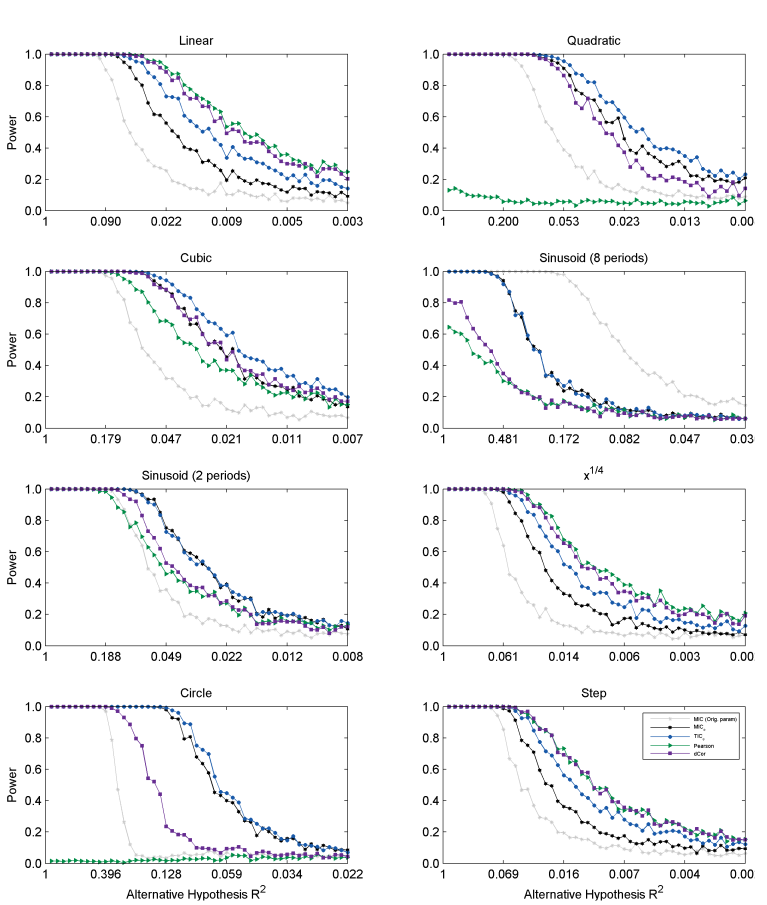
\includegraphics[width= \textwidth]{reshef_2016_fig5.png}
            \caption{Comparaci\'on del poder de prueba de independencia basado en $TIC_e$ (azul) con $MIC$ con par\'ametros predeterminados (gris), $MIC_e$ con los mismos par\'ametros que $TIC_e$ (negro), correlaci\'on de distancia (p\'urpura) y el coeficiente de correlaci\'on de Pearson (verde) en varios tipos de relaciones de hip\'otesis alternativas elegidos por Simon y Tibshirani (2012 \cite{SimonTibshirani}).}
            \label{reshef_2016_f5}
        \end{figure}
    
    
\newpage    
    % ---------------------------------------------------------------------------------------
\section[Covarianza y Correlaci\'on por Distancia]{Covarianza y Correlaci\'on por Distancia}

\subsection{Sobre el coeficiente}

En la secci\'on anterior, discutimos el MIC y el TIC, dos medidas de asociaci\'on utilizadas para cuantificar relaciones no lineales entre datos, pero no es la \'unica, y de hecho es cr\'iticada por tener algunas falencias al momento de detectar la fuerza entre relaciones \cite{SimonTibshirani}. Por esto tambi\'en buscamos otra medida que nos ayudar\'a a complementar el an\'alisis de asociaci\'on entre variables, y por esto en este cap\'itulo estudiaremos la Covarianza y Correlaci\'on por Distancia.

La Covarianza por Distancia (cCor) y la Correlaci\'on por distancia (dCor) fueron propuestas por Sz\'ekely, Rizzo, y Bakirov en su trabajo \textit{''Measuring and testing independence by correlation of distances''} (2007) \cite{Szekely2007}, posteriormente tambi\'en propusieton la Covarianza por Distancia Browniana en su trabajo \textit{''Brownian Distance Covariance''} (2009) \cite{Szekely2009}, en donde tambi\'en se demostr\'o que esta coincide con la Covarianza por Distancia tradicional.

Estas son medidas de asociaci\'on no param\'etricas que buscan encontrar relaciones no lineales entre dos conjuntos de datos, en particular establecer una forma de caracterizar independenc\'ia entre dos distribuci\'ones. Dado esto es importante recalcar que, para distribuci\'on de primer momento fin\'ito, la Correlaci\'on por distancia ($\mathcal{R}$) generaliza la idea de correalci\'on en dos formas:

\begin{enumerate}
	\item $\mathcal{R}(X,Y)$ est\'a definido para $X,Y$ de dimensi\'on aleatoria.
	\item $\mathcal{R}(X,Y) = 0$ caracteriza la independenc\'a de $X$ e $Y$.	 
\end{enumerate}

La primera de estas afirmaciones es importante, ya que nos permite utulizar esta medida para comparar im\'agenes sin mayor problema, de todas formas en la secci\'on \ref{chap5} estudiaremos como adaptar est\'as medidas para im\'agnes. En esta secci\'on definiremos estos 3 coeficientes, la relaci\'on entre ellos y verificaremos la afirmaciones realizadas m\'as arriba, para esto comenzaremos con las definiciones. 

\subsection{Definiciones}

Sean $X$ en $\R^p$ y $Y$ en $\R^q$ vectores aleatorios, donde $p$ y $q$ son enteros positivos. Las funciones en min\'uscula $f_X$ y $f_Y$ se utilizarán para denotar las funciones caracter\'isticas de $X$ y $Y$, respectivamente, y su funci\'on caracter\'istica conjunta se denota como $f_{X, Y}$. 

\begin{defn}[Covarianza por distancia]
	La Covarianza por distancia (dCov) entre los vectores aleatorios $X$ e $Y$ con primeros momentos finitos es el n\'umero no negativo $\mathcal{V}(X, Y)$ definido por:
	\begin{equation}
		\begin{aligned}\label{dcov_formula}
			\mathcal{V}^2(X, Y) & =\left\|f_{X, Y}(t, s)-f_X(t) f_Y(s)\right\|^2 \\
			& =\frac{1}{c_p c_q} \int_{\R^{p+q}} \frac{\left|f_{X, Y}(t, s)-f_X(t) f_Y(s)\right|^2}{|t|_p^{1+p}|s|_q^{1+q}} d t d s .
			\end{aligned}
	\end{equation}

	\end{defn}

	Similarmente, la Varianza por distancia (dVar) se define como la raiz cuadrada:

	$$
	\mathcal{V}^2(X)=\mathcal{V}^2(X, X)=\left\|f_{X, X}(t, s)-f_X(t) f_X(s)\right\|^2 .
	$$

	Por definici\'on de la norma $\|\cdot\|$, es claro que  $\mathcal{V}(X, Y) \geq 0$ y $\mathcal{V}(X, Y)=0$ si y solo si $X$ e $Y$ son indepentes.

	\begin{defn} [Correlaci\'on por distancia]
		La correlaci\'on por distancia (dCor) entre los vectores aleatorios $X$ e $Y$ con primer momento finito es el n\'unero no negtivo $\mathcal{R}(X, Y)$ definido por:
		$$
		\mathcal{R}^2(X, Y)= \begin{cases}\frac{\mathcal{V}^2(X, Y)}{\sqrt{\mathcal{V}^2(X) \mathcal{V}^2(Y)}}, & \mathcal{V}^2(X) \mathcal{V}^2(Y)>0 \\ 0, & \mathcal{V}^2(X) \mathcal{V}^2(Y)=0\end{cases}.
		$$

	Algunas propiedades de $\mathcal{R}$ an\'alogo a $\rho$ ser\'an revisadas m\'as adelante. 
	\end{defn}

	Ahora, para el caso muestral, definimos los estad\'isticos de distancia de la siguiente forma. Para una muestra aleatoria $(\mathbf{X}, \mathbf{Y})=\left\{\left(X_k, Y_k\right): k=1, \ldots, n\right\}$ de $n$ ventores aleatorios $(X, Y)$ i.i.d., calculamos las matrices de distancia euclideana  $\left(a_{k l}\right)=\left(\left|X_k-X_l\right|_p\right)$ y $\left(b_{k l}\right)=\left(\left|Y_k-Y_l\right|_q\right)$. Definimos:

	$$
	A_{k l}=a_{k l}-\bar{a}_{k .}-\bar{a}_{. l}+\bar{a}_{. .}, \quad k, l=1, \ldots, n,
	$$
	donde
	$$
	\bar{a}_{k .}=\frac{1}{n} \sum_{l=1}^n a_{k l}, \quad \bar{a}_{. l},=\frac{1}{n} \sum_{k=1}^n a_{k l}, \quad \bar{a}_{. .}=\frac{1}{n^2} \sum_{k, l=1}^n a_{k l} .
	$$
	
	De forma similar, definimos $B_{k l}=b_{k l}-\bar{b}_{k .}-\bar{b}_{\cdot l}+\bar{b}_{. .}$, para $k, l=1, \ldots, n$.

	\begin{defn}[Covarianza y Correlaci\'on por distancia muestral]
		La no negativa Covarianza por distancia muestral $\mathcal{V}_n(\mathbf{X}, \mathbf{Y})$ y la Correlaci\'on por distancia muestral $\mathcal{R}_n(\mathbf{X}, \mathbf{Y})$ estan definidas por
		$$
		\mathcal{V}_n^2(\mathbf{X}, \mathbf{Y})=\frac{1}{n^2} \sum_{k, l=1}^n A_{k l} B_{k l},
		$$
		y
		$$
		\mathcal{R}_n^2(\mathbf{X}, \mathbf{Y})= \begin{cases}\frac{\mathcal{V}_n^2(\mathbf{X}, \mathbf{Y})}{\sqrt{\mathcal{V}_n^2(\mathbf{X}) \mathcal{V}_n^2(\mathbf{Y})}}, & \mathcal{V}_n^2(\mathbf{X}) \mathcal{V}_n^2(\mathbf{Y})>0 \\ 0, & \mathcal{V}_n^2(\mathbf{X}) \mathcal{V}_n^2(\mathbf{Y})=0\end{cases},
		$$
		respectivamente. Adem\'as la Varianza por distancia muestral $\mathcal{V}_n(\mathbf{X})$ est\'a definida por
		$$
		\mathcal{V}_n^2(\mathbf{X})=\mathcal{V}_n^2(\mathbf{X}, \mathbf{X})=\frac{1}{n^2} \sum_{k, l=1}^n A_{k l}^2 .
		$$
	\end{defn}

	Por ultimo, plantearemos los siguientes teoremas que nos entregan  propiedades importantes de la Correlaci\'on por distancia:

	\begin{thm}
		Si $(\mathbf{X}, \mathbf{Y})$ es una muestra aleatoria del vector aleatorio $(X, Y)$, entonces
		$$
		\mathcal{V}n^2(\mathbf{X}, \mathbf{Y})=\left\|f{X, Y}^n(t, s)-f_X^n(t) f_Y^n(s)\right\|^2 .
		$$
	\end{thm}
	\begin{thm}
		Si $E|X|_p<\infty$ and $E|Y|_q<\infty$, entonces casi seguramente
		$$
		\lim _{n \rightarrow \infty} \mathcal{V}_n(\mathbf{X}, \mathbf{Y})=\mathcal{V}(X, Y) .
		$$
	\end{thm}
	
	\begin{cor}
		If $E\left(|X|_p+|Y|_q\right)<\infty$, then almost surely
		$$
		\lim _{n \rightarrow \infty} \mathcal{R}_n^2(\mathbf{X}, \mathbf{Y})=\mathcal{R}^2(X, Y) \text {. }
		$$
	\end{cor}
	\begin{thm}\label{thm3_brcov}
		Para vectores aleatorios $X \in \mathbb{R}^p$ y $Y \in \mathbb{R}^q$ tal que $E\left(|X|_p+\right.$ $\left.|Y|_q\right)<\infty$, se tienen las siguientes propiedades:
		\begin{enumerate}
			\item $0 \leq \mathcal{R}(X, Y) \leq 1$, y $\mathcal{R}=0$ si y solo si $X$ e $Y$ son independientes.
			\item $\mathcal{V}\left(a_1+b_1 C_1 X, a_2+b_2 C_2 Y\right)=\sqrt{\left|b_1 b_2\right|} \mathcal{V}(X, Y)$, para todos los vectores constantes $a_1 \in \mathbb{R}^p, a_2 \in \mathbb{R}^q$, escalares $b_1, b_2$ y matrices ortogonales $C_1, C_2$ en $\mathbb{R}^p$ y $\mathbb{R}^q$, respectivamente.	
			\item Si el vector aleatorio $\left(X_1, Y_1\right)$ es ind. del vector aleatorio $\left(X_2, Y_2\right)$, se tiene
			 $$
			\mathcal{V}\left(X_1+X_2, Y_1+Y_2\right) \leq \mathcal{V}\left(X_1, Y_1\right)+\mathcal{V}\left(X_2, Y_2\right) .
			$$
			La igualdad se cumple si y solo si $X_1$ e $Y_1$ son constantes, o $X_2$ e $Y_2$ son constantes, o $X_1, X_2, Y_1, Y_2$ son mutuamente independientes.

			\item $\mathcal{V}(X)=0$ implica que $X=E[X]$, casi seguramente.
			\item $\mathcal{V}(a+b C X)=|b| \mathcal{V}(X)$, para todos los vectores constantes $a$ en $\mathbb{R}^p$, escalares $b$, y matrices ortogonales $p \times p$ $C$.
			\item Si $X$ e $Y$ son independientes, entonces $\mathcal{V}(X+Y) \leq \mathcal{V}(X)+\mathcal{V}(Y)$. La igualdad se cumple si y solo si uno de los vectores aleatorios $X$ o $Y$ es constante.
		\end{enumerate}
	\end{thm}
	\begin{thm}
	\begin{enumerate}
		\item $\mathcal{V}_n(\mathbf{X}, \mathbf{Y}) \geq 0$.
		\item $\mathcal{V}_n(\mathbf{X})=0$ si y solo si cada observaci\'on de la muestra es id\'entica.
		\item $0 \leq \mathcal{R}_n(\mathbf{X}, \mathbf{Y}) \leq 1$.
		\item $\mathcal{R}_n(\mathbf{X}, \mathbf{Y})=1$ implica que las dimensiones de los subespacios lineales generados por $\mathbf{X}$ y $\mathbf{Y}$ respectivamente son casi seguramente iguales, y si asumimos que estos subespacios son iguales, entonces en este subespacio
		\item $$
		\mathbf{Y}=a+b \mathbf{X} C,
		$$
		para alg\'un vector $a$, n\'umero real no nulo $b$, y matriz ortogonal $C$.
	\end{enumerate}	
	\end{thm}
	demostraci\'ones de todos estos teoremas pueden ser encontrados en Szekely y Rizzo (2009) \cite{Szekely2009}.


	\subsection{Covarianza Browniana}
		
		Para introducir la noci\'on de covarianza browniana, comenzaremos considerando la covarianza cuadrada del producto-momento. Recordemos que una variable prima $X'$ denota una copia independiente e id\'enticamente distribuida (i.i.d.) del símbolo no prima $X$. Para dos variables aleatorias continuas de valores reales, el cuadrado de su covarianza clásica es:

		$$\E[(X-\E(X))(Y-\E(Y))] = \E[(X-\E(X))(X'-\E(X'))(Y-\E(Y))(Y'-\E(Y'))]	$$

		Ahora generalizamos la covarianza al cuadrado y definimos el cuadrado de la covarianza condicional, dadas dos procesos estocásticos de valores reales, $U(\circ)$ y $V(*)$. Obtenemos un resultado interesante cuando U y V son procesos de Wiener independientes.


		Primero, para centrar la variable aleatoria $X$ en la covarianza condicional, necesitamos la siguiente definici\'on. Sea $X$ una variable aleatoria de valores reales y $\{U(t): t \in \R\}$ un proceso estoc\'astico de valores reales, independiente de $X$. La versi\'on centrada de $X$ respecto a $U$ se define por:

		$$
		X_U = U(X)-\int_{-\infty}^{\infty}U(t)dF_X(t)=U(X)-\E[U(X)|U],
		$$

		siempre que la esperanza condicional exista. Notemos que, si $id$ es la identidad, $X_{id}=X-\E[X]$. 

		Ahora, sea $\mathcal{W}$ un movimiento Browniano/Wiener de una dimensi\'on en ambos lados con esperanza cero y funci\'on de covarianza.
		\begin{equation}\label{brw_covariamce}
			|s|+|t|-|s-t|=2\min(s.t)
		\end{equation}
			

		Esto es dos veces la covarianza estandar para un proceso Wiener. Pero en adelante el factor de dos nos simplificar\'a algunos calculos, por lo que en el resto de la secci\'on asumiermos esta funci\'on de covarianza \ref{brw_covariamce} para $\mathcal{W}$. Ya con esto, podemos definir la Covarianza Browniana 

		\begin{defn}[Covarianza Browniana]
			La Covarianza Browniana (o covarianza Wiener) de dos variables aleatorias con valores reales $X$ e $Y$, con segundos monetos fin\'itos es el n\'umero no negativo definido por su cuadrado:
			\begin{equation}\label{brw_cov}
				\mathcal{W}^2(X,Y)={Cov}_{{W}^2}(X,Y)=\E[X_{W}X'_{W}Y_{W'}Y'_{W'}],
			\end{equation}

			donde $({W},{W'})$ no dependen de $(X,X',Y.Y')$.
		\end{defn}

		Tomemos en cuenta que si ${W}$ en ${Cov}_{{W}^2}$ es reemplazada por la funci\'on identidad (no aleatoria) $id$, entonces ${Cov}_{id}(X, Y) = |{Cov}(X, Y)| = |\sigma_{X,Y}|$, el valor absoluto de la covarianza del producto-momento de Pearson. Mientras que la covarianza del producto-momento estandarizada, la correlación de Pearson ($\rho$), mide el grado de relaci\'on lineal entre dos variables con valores reales, veremos que la covarianza estandarizada de Brownian mide el grado de todos los tipos posibles de relaciones entre dos variables aleatorias con valores reales.

		La definición de ${Cov}_{{W}^2}$ se puede extender a procesos aleatorios en dimensiones superiores de la siguiente manera. Si $X$ es una variable aleatoria con valores en $\R^p$ y $U(s)$ es un proceso aleatorio (campo aleatorio) definido para todos los $s \in \R^p$ e independiente de $X$, define la versión centrada en $U$ de $X$ como

		$$
			X_U=\E(X)-\E[U(X)|U]
		$$
		siempre que la expectativa condicional exista.

		\begin{defn}
			Si $X$ es un vector aleatorio con valores en $\R^p$ y $Y$ es un vector aleatorio con valores en $\R^q$, y $U(s)$ y $V(t)$ son procesos aleatorios, definamos para todo $s\in\R^p$, $t\in\R^q$, entonces la covarianza (U,V) de $X$ e $Y$ es el n\'umero no negativo definido por su cuadrado:
			\begin{equation}\label{eq_35_brcov}
				{Cov}^2_{(U,V)}(X,Y) = \E[X_U X'_U Y_V Y'_V],
			\end{equation}
				
			siempre que el lado derecho sea positivo y finito.
		\end{defn}

		En particular, si ${W}$ y ${W'}$ son procesos brownianos con funci\'on de covarianza \ref{brw_covariamce} en $\R^p$ y $\R^q$ respectivamente, la Covarianza Browniana de $X$ e $Y$ esta definida por:

		\begin{equation}
			\mathcal{W}^2(X,Y) = Cov^2_W(X,Y) = Cov^2_{W,W'}(X,Y).
		\end{equation}

		De la misma forma, para variables aleatorias con varianza finita podemos definir la Varianza Browniana:

		\begin{equation}
			\mathcal{W}(X) = Cov_W(X) = Cov_{W}(X,X).
		\end{equation}
		
		Y con esto, podemos definir la correlaci\'on Browniana:
		
		\begin{defn}[Correlaci\'on Browniana]
			Definimos la correalci\'on Browniana de dos variables aleatorias con valores reales $X$ e $Y$ con segundos momentos finitos como:
			\begin{equation}	
				Cor_W(X,Y) = \frac{\mathcal{W}}{\sqrt[]{\mathcal{W}(X)\mathcal{W}(Y)}},
			\end{equation}
			siempre que el denominador no sea 0; otro caso $Cor_W(X,Y) = 0$.
		\end{defn}

		Ahora, solo nos queda probar que $Cov_W(X,Y)$ existe para vectores aleatorios de segundos momentos finitos, y con esto derivar la Covarianza Browniana. Para esto, tenemos el siguiente teorema:

		\begin{thm}\label{thm_exists_cov_browniana}
			Si $X$ es un vector aleatorio con valores en $\R^p$, e $Y$ es un vector aleatorio con valores en $\R^q$, y $\E(|X|^2+|Y|^2)>\infty$, entonces $\E[X_{W}X'_{W}Y_{W'}Y'_{W'}]$ es no negativo y finito, y:
			\begin{align}
				\mathcal{W}^2(X,Y) &= \E[X_{W}X'_{W}Y_{W'}Y'_{W'}]\\
								   &= \E|X-X'||Y-Y'| + \E|X-X'|\E|Y-Y'| - \label{cov_browniana_exists} \\ 
								   &\qquad - \E|X-X'||Y-Y''|\E|X-X''||Y-Y'|,\label{eq_37_brcov}
 			\end{align}
			donde $(X,Y)$, $(X',Y')$, y $(X'',Y'')$ son iid.
		\end{thm}
		\begin{proof}
			Notemos que
			$$
			\begin{aligned}
			E\left[X_W X_W^{\prime} Y_{W^{\prime}} Y_{W^{\prime}}^{\prime}\right] & =E\left[E\left(X_W Y_{W^{\prime}} X_W^{\prime} Y_{W^{\prime}}^{\prime} \mid W, W^{\prime}\right)\right] \\
			& =E\left[E\left(X_W Y_{W^{\prime}} \mid W, W^{\prime}\right) E\left(X_W^{\prime} Y_{W^{\prime}}^{\prime} \mid W, W^{\prime}\right)\right] \\
			& =E\left[E\left(X_W Y_{W^{\prime}} \mid W, W^{\prime}\right)\right]^2,
			\end{aligned}
			$$
			y esto es siempre no negativo. Para finitud, es suficiente demostrar que todos los factores en la definici\'on de  $\operatorname{Cov}_W(X, Y)$ tienen cuartos momentos finitos. La ecuaci\'on \ref{cov_browniana_exists} se basa en la forma especial de la funci\'on de covarianza de \ref{brw_covariamce} de $W$. El resto de la demostraci\'on se puede encontrar en el ap\'endice de /Szehely and Rizzo (2009)\cite{Szekely2009}.	
		\end{proof}

	\subsection{Equivalencia entre covarianzas}
	
	Ahora estudiaremos la equivalencia entre la Covarianza por distancia y la Covarianza Browniana. Pero antes de esto necesitamos plantear el siguiente lema:

	\begin{lem}\label{lemma_1_brcov}
		Si $0<\alpha<2$, entonces para todo $x$ en $\R^d$
		$$
		\int_{\R^d} \frac{1-\cos \langle t, x\rangle}{|t|_d^{d+\alpha}} d t=C(d, \alpha)|x|_d^\alpha,
		$$
		donde
		$$
		C(d, \alpha)=\frac{2 \pi^{d / 2} \Gamma(1-\alpha / 2)}{\alpha 2^\alpha \Gamma((d+\alpha) / 2)},
		$$
		y $\Gamma(\cdot)$ es la funci\'on completea gamma. Las integrales en 0 y $\infty$ se entienden en el sentido de valor principal: $\lim_{\varepsilon \rightarrow 0} \int_{\R^d \backslash\left\{\varepsilon B+\varepsilon^{-1} B^c\right\}}$, donde $B$ es la bola unitaria (centrada en 0) en $\R^d$ y $B^c$ es el complemento de $B$.
	\end{lem}
	Una demostraci\'on de este lemma puede ser entontrada en Székely and Rizzo (2007) \cite{Szekely2007}. El Lemma \ref{lemma_1_brcov}
	sugiere que la funci\'on de pesos
	\begin{equation}\label{eq_23_brcov}
	w(t, s ; \alpha)=\left(\left.\left.C(p, \alpha) C(q, \alpha)|t|_p^{p+\alpha}\right|s\right|_q ^{q+\alpha}\right)^{-1}, \quad 0<\alpha<2 .	
	\end{equation}

	En el caso m\'as simple correspondiente a $\alpha=1$ y norma euclidiana $|x|$,
	\begin{equation}\label{eq_24_brcov}
		w(t, s)=\left(c_p c_q|t|_p^{1+p}|s|_q^{1+q}\right)^{-1},
		\end{equation}
	
	donde,
	\begin{equation}\label{eq_25_brcov}
		c_d=C(d, 1)=\frac{\pi^{(1+d) / 2}}{\Gamma((1+d) / 2)} .
	\end{equation}
	
	(La constante $2 c_d$ es el \'area de la esfera unitaria en $\R^{d+1}$).
	\begin{rem}
		El Lemma \ref{lemma_1_brcov} es aplicado para evaluar el integrando en \ref{dcov_formula} para las funciones de peso \ref{eq_23_brcov} y \ref{eq_24_brcov}. Por ejemplo, si $\alpha=1$ \ref{eq_24_brcov}, entonces por el Lemma \ref{lemma_1_brcov} existen constantes $c_p$ y $c_q$ tal que para $X$ en $\R^p$ y $Y$ en $\R^q$,
		$$
		\begin{gathered}
		\int_{\mathbb{R}^p} \frac{1-\exp \{i\langle t, X\rangle\}}{|t|p^{1+p}} d t=c_p|X|_p, \quad \int{\mathbb{R}^q} \frac{1-\exp \{i\langle s, Y\rangle\}}{|s|_q^{1+q}} d s=c_q|Y|_q, \\
		\int_{\mathbb{R}^p} \int_{\mathbb{R}^q} \frac{1-\exp \{i\langle t, X\rangle+i\langle s, Y\rangle\}}{|t|_p^{1+p}|s|_q^{1+q}} d t d s=c_p c_q|X|_p|Y|_q
		\end{gathered}
		$$
	\end{rem}
	
	Ya con esto, podemos pasar el resultado principal de esta secci\'on, con el siguiente teorema.
	

	\begin{thm}\label{thm_8_brcov}
		Para un $X \in \R^p, Y \in \R^q$ arbitrario, con segundos momentos finitos
			$$
			\mathcal{W}(X, Y)=\mathcal{V}(X, Y) .
			$$
			\end{thm}
	
	\begin{proof}
		
	Proof. Ambos $\mathcal{V}$ y $\mathcal{W}$ son no negativos, por tanto, basta por demostrar que sus cuadrados coinciden. Para esto, primero notemos Lemma \ref{lemma_1_brcov} puede ser aplicado para evaluar $\mathcal{V}^2(X, Y)$. En el numerador de la integral tenemos t\'erminos como:
	
	$$
	E\left[\cos \left\langle X-X^{\prime}, t\right\rangle \cos \left\langle Y-Y^{\prime}, s\right\rangle\right],
	$$

	donde $X, X^{\prime}$ son i.i.d. y $Y, Y^{\prime}$ son i.i.d. Ahora, aplicando la identidad:
	$$
	\cos u \cos v=1-(1-\cos u)-(1-\cos v)+(1-\cos u)(1-\cos v)
	$$
	y el Lemma \ref{lemma_1_brcov} para simplificar el integrando. Despu\'es de cancelar en el numerador del integrando, queda por evaluar integrales del tipo:

	$$
	\begin{aligned}
	& E \int_{\R^{p+q}} \frac{\left.\left[1-\cos \left\langle X-X^{\prime}, t\right\rangle\right]\left[1-\cos \left\langle Y-Y^{\prime}, s\right\rangle\right)\right]}{|t|^{1+p}|s|^{1+q}} d t d s \\
	& \quad=E\left[\int_{\R^p} \frac{1-\cos \left\langle X-X^{\prime}, t\right\rangle}{|t|^{1+p}} d t \times \int_{\R^q} \frac{1-\cos \left\langle Y-Y^{\prime}, s\right\rangle}{|s|^{1+q}} d s\right] \\
	& =c_p c_q E\left|X-X^{\prime}\right| E\left|Y-Y^{\prime}\right|
	\end{aligned}
	$$
	Luego de esto, y simplificando, obtenemos:
	$$
	\begin{aligned}
	\mathcal{V}^2(X, Y)= & E\left|X-X^{\prime}\right|\left|Y-Y^{\prime}\right|+E\left|X-X^{\prime}\right| E\left|Y-Y^{\prime}\right| \\
	& -E\left|X-X^{\prime}\right|\left|Y-Y^{\prime \prime}\right|-E\left|X-X^{\prime \prime}\right|\left|Y-Y^{\prime}\right|,
	\end{aligned}
	$$
	y esta es exactamente igual a la expresi\'on \ref{eq_37_brcov} obtenida para $\mathcal{W}^2(X, Y)$ en el Teorema \ref{thm_exists_cov_browniana}.
	\end{proof}

	Como corolario del Teorema \ref{thm_8_brcov}, tenemos que las propiedades de la Covarianza Browniana para vectores aleatorios $X$ e $Y$ con segundos momentos finitos son las mismas propiedades establecidas para la Covarianza por distancia $\mathcal{V}(X, Y)$ en el Teorema \ref{thm3_brcov}.
	
	El sorpredente resultado de que la Covarianza Browniana es igual a la Covarianza por distancia, exactamente como se define en \ref{dcov_formula} para $X \in \R^p$ e $Y \in \R^q$, es paralelo a un caso especial familiar cuando $p=q=1$. Para bivariados $(X, Y)$ encontramos que $\mathcal{R}(X, Y)$ es un contraparte natural del valor absoluto de la correlaci\'on de Pearson. Es decir, si en \ref{eq_35_brcov} $U$ y $V$ son la funci\'on no aleatoria m\'as simple $id$, entonces obtenemos el cuadrado de la covarianza de Pearson $\sigma_{X, Y}^2$. Luego, si consideramos los procesos aleatorios m\'as fundamentales, $U=W$ y $V=W^{\prime}$, obtenemos el cuadrado de la covarianza por distancia, $\mathcal{V}^2(X, Y)$.


    \section{Ejemplos}

    Ya con los coeficientes claros, podemos revisar un ejemplo r\'apido de estos. Para esto usaremos "The Datasaurus Dozon", un conjutno de datos propuesto por Justin Matejka y George Fitzmaurice (2017) \cite{datasaurus}. Este conjunto de datos nos presenta con 13 realciones, visibles en la Figura \ref{datasaurus_fig}, las cuales todas poseen los mismos valores para estad\'isticos descriptivos comunos (Promedio Marginal, Desviac\'on Estandar Marginal, y Correlaci\'on de Pearson), pero son claramente visualmente distinos.

    \begin{figure} 
        \centering
        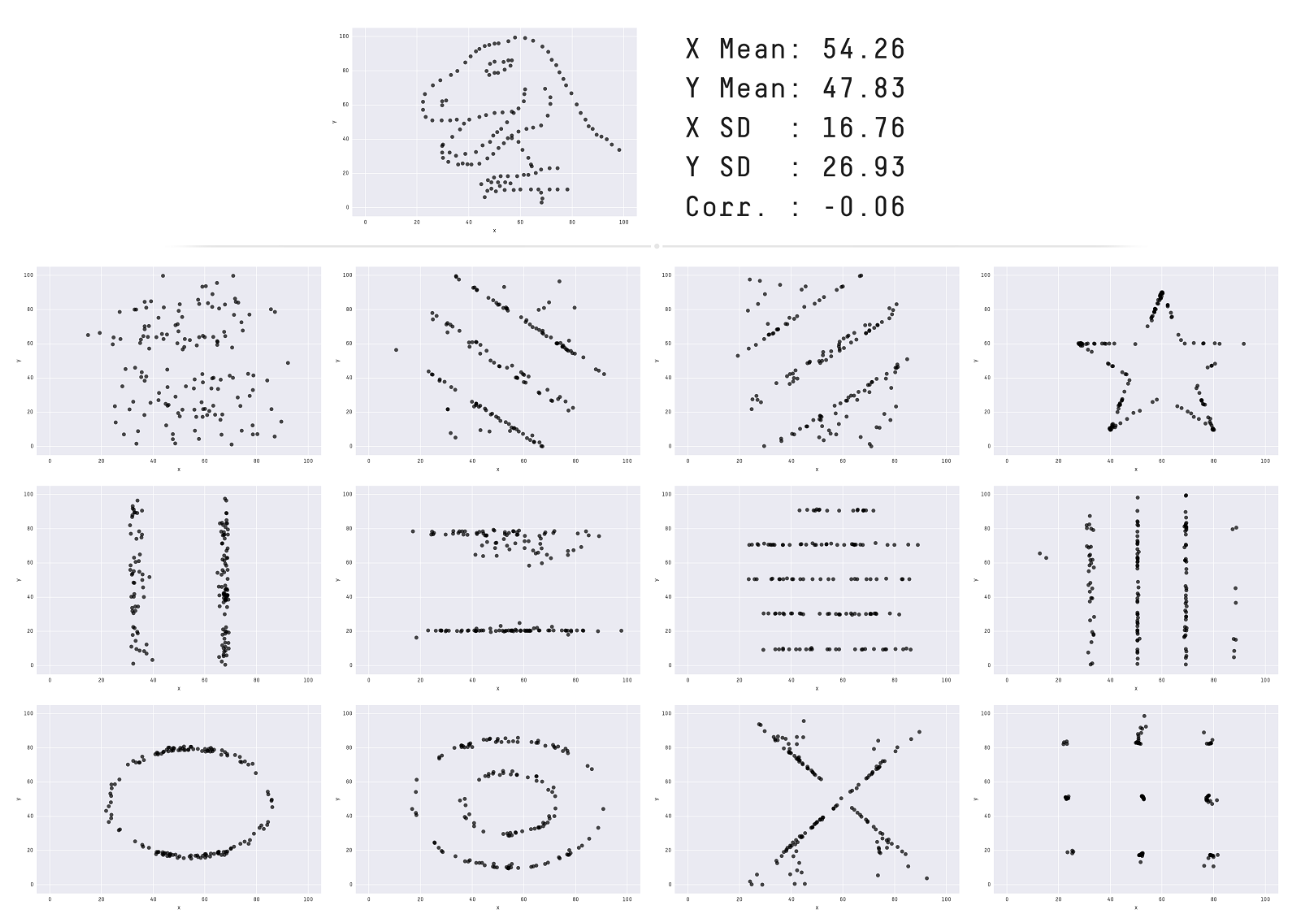
\includegraphics[width=\textwidth]{datasaurusdozon.png}
        \caption{The Datasaurus Dozon", a pesar de compartir los mismos estad\'isticos descriptivos, son visualmente distintos.}
        \label{datasaurus_fig}
    \end{figure}

    De particular interes para nosotros es el valor de la correlaci\'on de Pearson de, que es b\'asicamente cero, lo que nos "deber\'ia" indicar que las relaciones son independientes, lo cuales claro con simplemente ver la Figura \ref{datasaurus_fig} que no es el caso. Es por esto que estos datos nos son de gran ayuda, dado que nos pueden dar una idea de como las correlaciones descritas pueden identificar otro tipo de relaci\'ones. Para esto revisemos la siguiente tabla \ref{tab:datsaurus} que contiene los valores de $MIC$ y $dCor$ para cada una de estas relaciones, en el mismo orden presentado en la Figura \ref{datasaurus_fig}.

    \begin{table}
        \label{tab:datsaurus}
        \centering
        \begin{tabular}{|l|lllll|}\hline
        Figura     & MIC  & TIC  & dCor & dCov & $\rho $   \\\hline
        Dino       & 0.18 & 2.67 & 0.16 & 2.36 & -0.064 \\
        Away       & 0.15 & 1.77 & 0.13 & 2.10 & -0.064 \\
        Slant Down & 0.21 & 2.87 & 0.16 & 2.29 & -0.069 \\
        Slant Up   & 0.22 & 3.37 & 0.19 & 2.79 & -0.069 \\
        Star       & 0.59 & 8.79 & 0.37 & 5.90 & -0.063 \\
        High Lines & 0.14 & 2.09 & 0.15 & 2.34 & -0.069 \\
        Wide Lines & 0.15 & 2.62 & 0.12 & 1.94 & -0.067 \\
        H Lines    & 0.14 & 2.07 & 0.15 & 2.30 & -0.062 \\
        V Lines    & 0.14 & 2.10 & 0.16 & 2.47 & -0.069 \\
        Circle     & 0.59 & 9.12 & 0.23 & 3.71 & -0.068 \\
        Bullseye   & 0.23 & 3.72 & 0.18 & 2.64 & -0.069 \\
        X Shape    & 0.48 & 7.76 & 0.20 & 3.28 & -0.066 \\
        Dots       & 0.31 & 3.89 & 0.13 & 2.13 & -0.060 \\\hline
        \end{tabular}
        \caption{Valores de $MIC$, $TIC$, $dCor$, $dCov$, y $\rho$ para cada una de las relaciones presentadas en la Figura \ref{datasaurus_fig}, en el mismo orden.}
    \end{table}
        

        

    Primero podemos confirmas que el coeficiente de pearson es similar y cercano a 0 en todos los casos, pero tanto el $MIC$ como el $dCor$ fueron capacez de detectar la relaci\'on entre las variables en cada uno de los casos, adem\'as tenemos altos valores de TIC en todos los casos, lo que nos indica que las una alta dependencia entre los valores. Nos llama la atenci\'on que ambas medidas, $MIC$ y $dCor$, nos dan valores similares, es m\'as, ambos est\'an de acuerdo en que la relaci\'on m\'as fuerte es la de la figura ''Star'', y detras la figura ''Circle'', que posee el mismo $MIC$ que la figura anterior, pero un $dCor$ m\'as bajo aunque siendo el segundo m\'as alto. 